\documentclass[../Article_Design_of_Experiment.tex]{subfiles}
\graphicspath{{\subfix{../Figures/}}}
\begin{document}
	
	\label{CH: Results}

	Both non-linear optimization problems are solved by applying a single-shooting technique to obtain the trajectory under the assumption of piece-wise constant controls. The CasADi framework is used as the interface for the IPOPT solver. Each simulation problem is solved multiple times, starting from different initial points, and the solution with the best score is considered the optimal solution.
	
	The first optimization problem was solved 69 times, starting from random initial guesses for the inlet temperature profile. The initial and final values of the objective function for each optimization are presented in Figure \ref{fig:DOE_T_OBJ}. It can be observed that multiple local minima are presented in the Figure. The global solution is selected from all the local solutions as the smallest local minima. 
	
	\begin{figure}[h!]
		\centering
		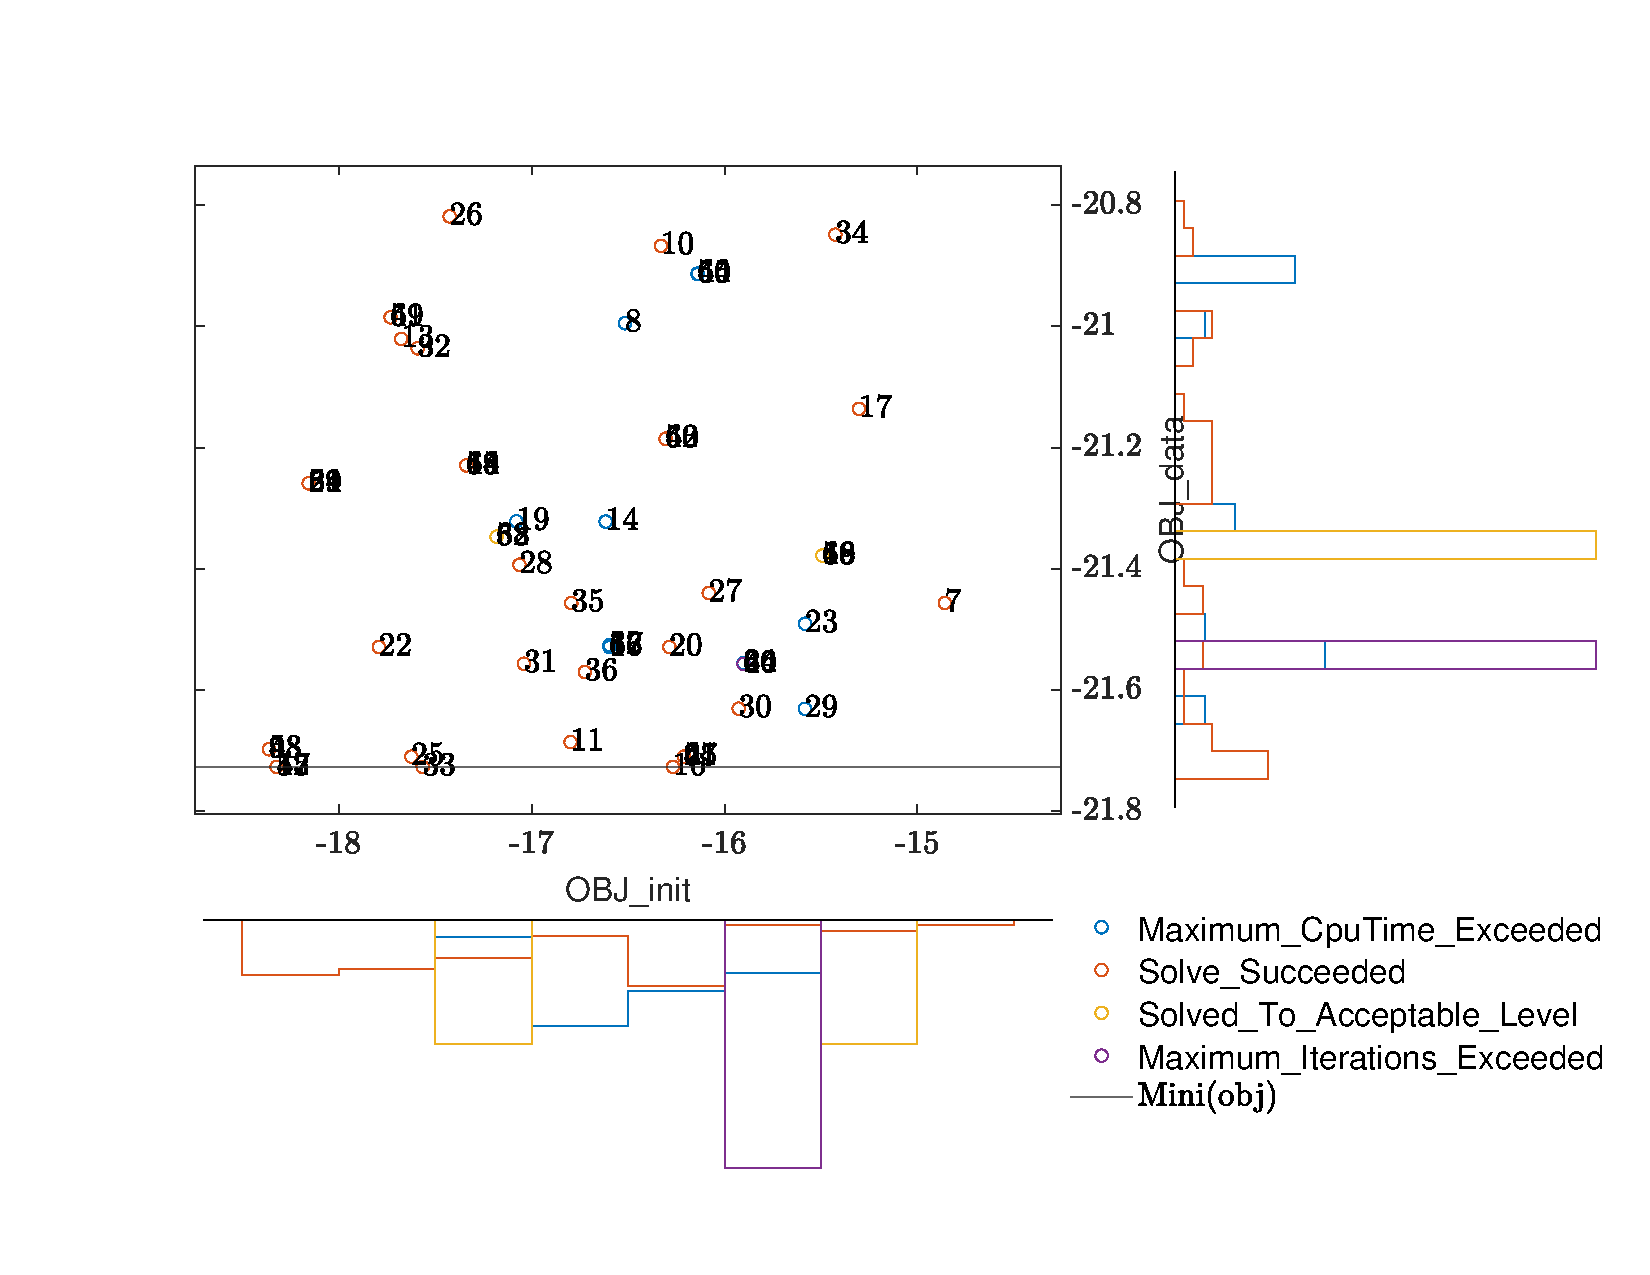
\includegraphics[trim = 3cm 1cm 0.5cm 2cm,clip,width=\columnwidth]{/Results_sensitivity/Multiple_shot_DOE_P250.pdf}
		\caption{Solution to the first DOE}
		\label{fig:DOE_T_OBJ}
	\end{figure}
	
	The inlet temperature profile, which corresponds to the solution of the first optimization problem, is presented in Figure \ref{fig:DOE_T_IN}. The general shape of the inlet temperature profile is similar to a square wave, with the second wave being wider than the first. The maximum and the minimum values correspond to the upper and the lower constraints for the inlet temperature. The similarity with a bang-bang controller should be mentioned, although the second wave has two intermediate values between the bounds.	
	
	Figure \ref{fig:DOE_T_OUT} shows the temperature profile at outlet of the extractor. The outlet profile differs from the inlet profile due to heat diffusion.
		
	\begin{figure}[h!]
		\centering
		\begin{subfigure}[b]{0.49\columnwidth}
			\centering
			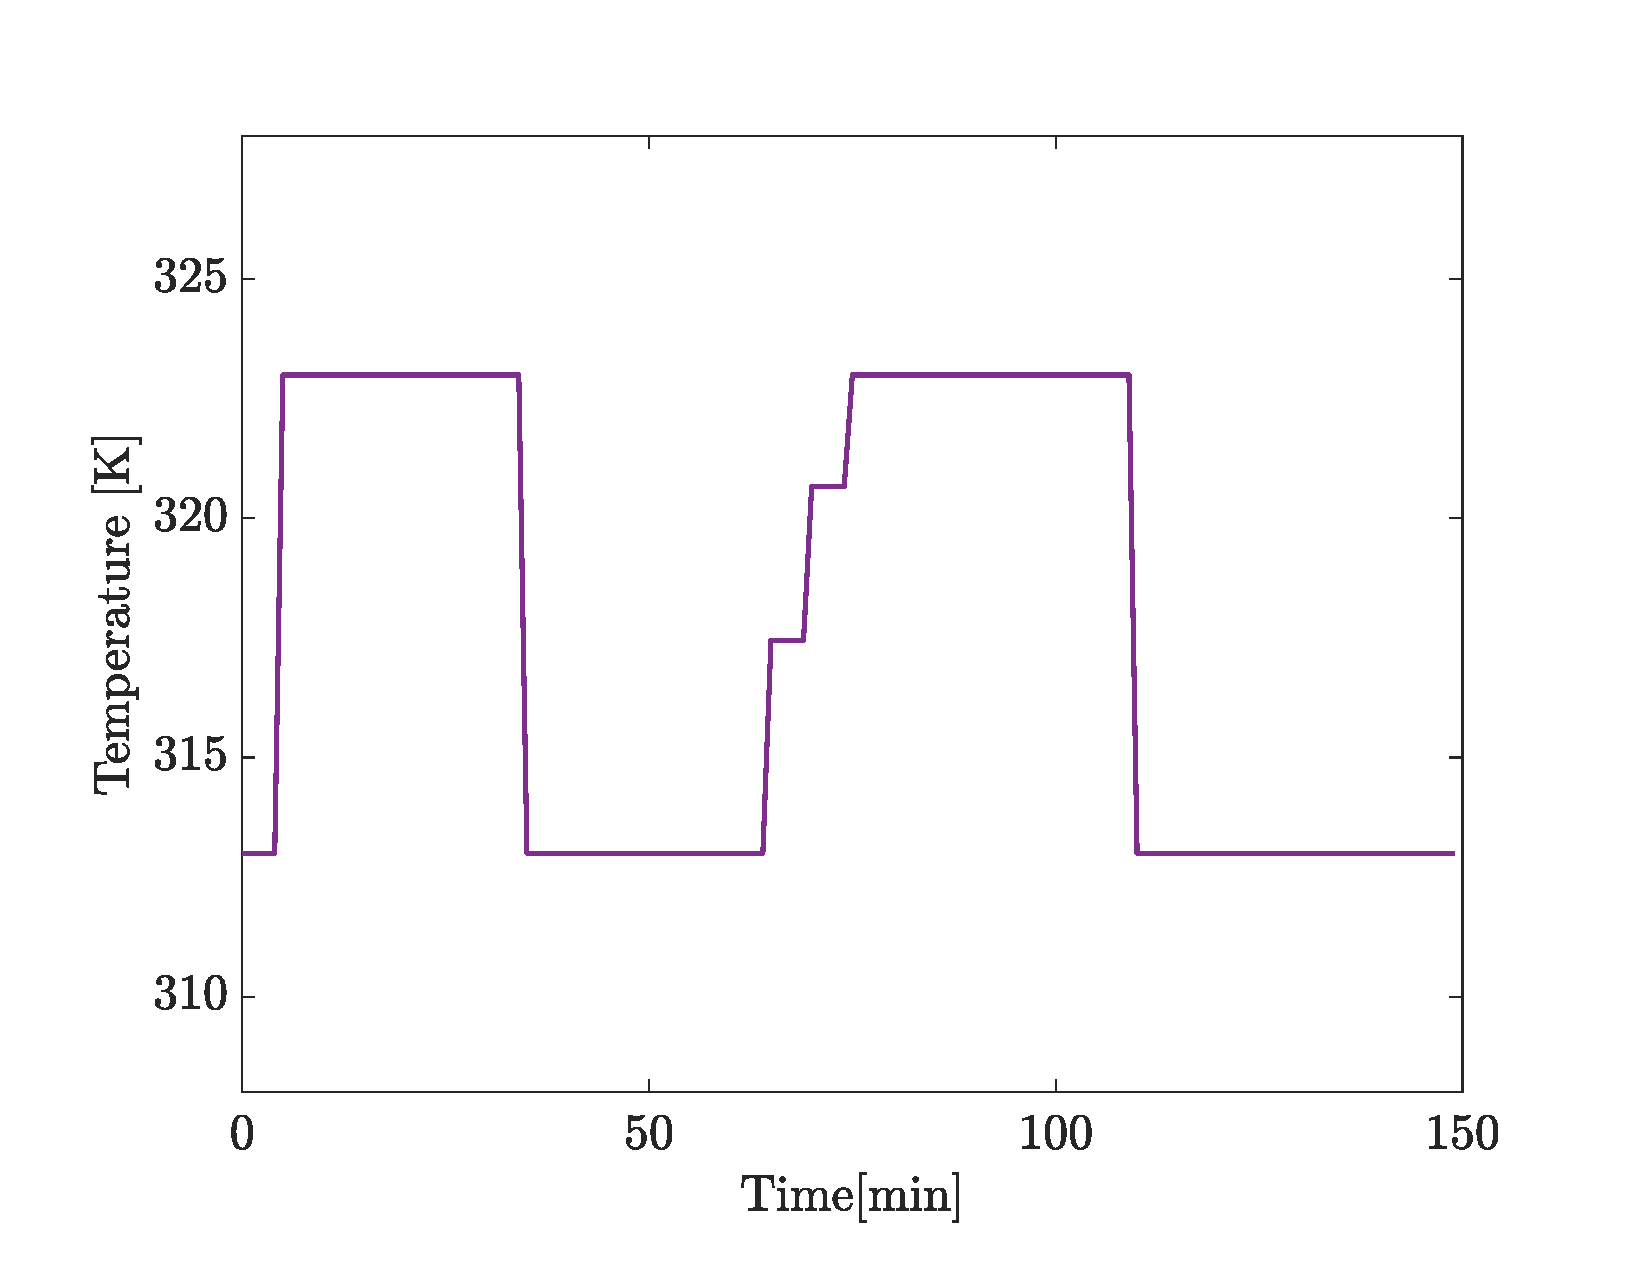
\includegraphics[trim = 1cm 1cm 2.5cm 2.0cm,clip,width=\columnwidth]{/Results_sensitivity/Best_T_in_P250.pdf}
			\caption{Inlet temperature profile}
			\label{fig:DOE_T_IN}
		\end{subfigure}
		\hfill
		\begin{subfigure}[b]{0.49\columnwidth}
			\centering
			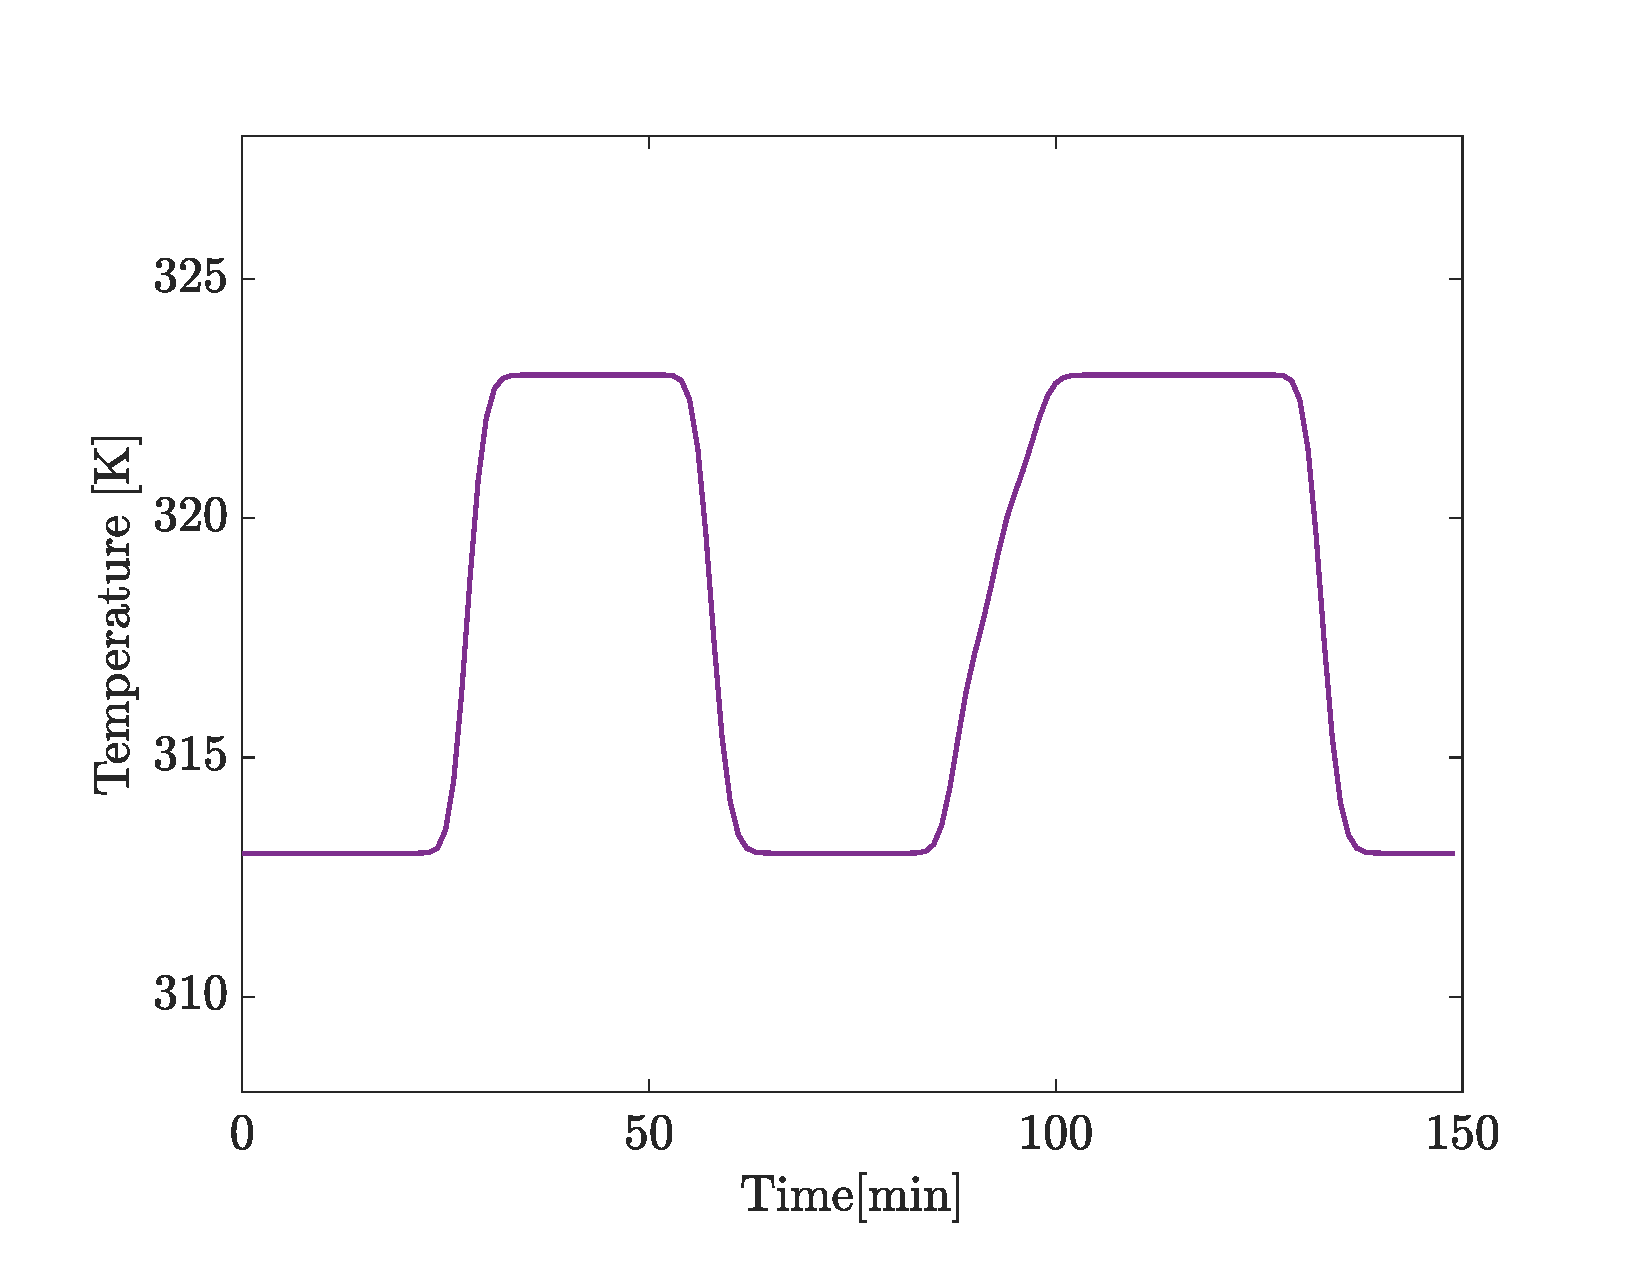
\includegraphics[trim = 1cm 1cm 2.5cm 2.0cm,clip,width=\columnwidth]{/Results_sensitivity/Best_T_out_P250.pdf}
			\caption{Outlet temperature profile}
			\label{fig:DOE_T_OUT}
		\end{subfigure}
		\caption{Global solution to the first optimization problem}
		\label{fig:DOE_T}
	\end{figure}
	
	
	
\end{document}


































